\documentclass[10pt,twocolumn]{article}
\usepackage[utf8]{inputenc}
\usepackage[T1]{fontenc}
\usepackage[english]{babel}
\usepackage[a4paper,margin=2cm]{geometry}
\usepackage{amsmath,amssymb}
\usepackage{graphicx}
\usepackage{booktabs}
\usepackage{hyperref}
\usepackage{xcolor}
\usepackage{natbib}
\bibliographystyle{plainnat}
\usepackage{caption}
\captionsetup{font=small, labelfont=bf}
\usepackage[capitalise,noabbrev]{cleveref}
\newcommand{\dd}{\mathrm{d}}

\hypersetup{colorlinks=true, linkcolor=blue!50!black, citecolor=blue!50!black,
  urlcolor=blue!50!black}

\title{\bfseries SleepArchitect:\\
  A free, no-login predictive sleep model from caffeine,\\
  alcohol, exercise, light, and chronotype}
\author{
  Anonymous Authors\\
  \texttt{\small sleeparchitect.local}
}
\date{May 2026}

\begin{document}
\twocolumn[
\begin{@twocolumnfalse}
\maketitle
\begin{abstract}
\noindent
Roughly 35\% of US adults report a sleep complaint, and a large
fraction of those complaints are modifiable -- caused by caffeine,
alcohol, evening light, exercise timing, or late meals.  Existing
consumer sleep apps (Oura, Whoop, Apple Health, Sleep Cycle,
AutoSleep) are uniformly retrospective: they tell you how you slept
last night.  We are not aware of any free open-source tool that
predicts \emph{tonight's} sleep from \emph{today's} caffeine,
alcohol, exercise, light, and meal timing.  Yet the underlying
quantitative model has existed for 40 years.  Borbely's two-process
model \citep{borbely1982two} couples a homeostatic Process S with a
circadian Process C; Skeldon et al. 2017 \citep{skeldon2017} gives a
practical implementation; Khalsa et al. 2003 \citep{khalsa2003} and
Zeitzer et al. 2000 \citep{zeitzer2000} provide the light
phase-response curve; Drake et al. 2013 \citep{drake2013}, Ebrahim
et al. 2013 \citep{ebrahim2013}, Stutz et al. 2019 \citep{stutz2019},
and Crispim 2011 \citep{crispim2011} provide caffeine, alcohol,
exercise, and meal modulators; Mallis et al. 2004 \citep{mallis2004}
gives the SAFTE alertness model for the next day's effectiveness.
We integrate all of these into \textsc{SleepArchitect}, an
open-source Python library and an elegant client-side web frontend
that takes an MCTQ chronotype and a day-in-progress and predicts
sleep onset latency, total sleep time, sleep efficiency,
REM/SWS/N1+N2 proportions, a 5-cycle hypnogram, a 24-hour
clock-face visualisation, the next day's SAFTE alertness curve, and
a ranked list of interventions.  Validation against 11 published
quantitative findings from the cited papers yields 11/11 within
published bands.  The single-page frontend (65\,KB raw /
18.7\,KB gzipped) runs in any browser with no backend, no login,
and no data collection.
\end{abstract}
\vspace{1em}
\end{@twocolumnfalse}
]

\section{Introduction}

The CDC reports that approximately 35\% of US adults sleep less than
7 hours per night and a similar fraction report at least one chronic
sleep complaint \citep{cdc2024sleep}.  A large portion of those
complaints are not pathological -- they are the predictable
consequence of \emph{modifiable} lifestyle factors: caffeine taken
too late, alcohol consumed in the evening, bright light exposure
near bedtime, exercise within 1\,hour of bed, large meals near
bedtime, or simply trying to sleep at a clock time that is
incompatible with one's chronotype.

Existing consumer sleep apps (Oura, Whoop, Apple Health,
Sleep Cycle, AutoSleep, Pillow, SleepCycle) measure sleep
retrospectively: they record what happened last night using
actigraphy, heart-rate variability, audio, or optional polysomnography
add-ons, and provide a sleep score that summarises the result.
Some apps offer post-hoc correlative analyses (``you sleep worse on
days when you drink alcohol'').  But none of these tools, to our
knowledge, attempts to \emph{predict} tonight's sleep from today's
caffeine, alcohol, exercise, light, and meal timing -- which is the
question users actually want to ask in the early evening.

This is striking because the necessary quantitative model has been
in the literature for forty years.  Borbely's seminal two-process
model \citep{borbely1982two} described sleep regulation in terms of
a homeostatic sleep pressure (Process S) and a circadian propensity
(Process C).  Daan, Beersma & Borbely 1984
\citep{daan1984timing} gave the standard parameters
$\tau_W = 18.2$\,h (wake rise) and $\tau_S = 4.2$\,h (sleep fall).
Skeldon et al. 2017 \citep{skeldon2017} provided a practical
implementation with light entrainment.  Phillips & Robinson 2007
\citep{phillips2007} extended the model to a neurally-grounded
flip-flop sleep-wake switch.  Adding the well-characterised modulators
-- caffeine PK and SWS effects \citep{carrillo2000,drake2013,clark2017},
alcohol PK and REM effects \citep{ebrahim2013}, exercise meta-analysis
\citep{stutz2019}, meal-timing effects \citep{crispim2011,iao2021},
light PRC + melatonin suppression
\citep{khalsa2003,zeitzer2000,brainard2001} -- gives a complete
personalised predictive model.  We bundle it as
\textsc{SleepArchitect}.

\paragraph{Contributions.}
\begin{enumerate}\setlength{\itemsep}{0pt}
\item An open-source Python library implementing Borbely two-process
$\rightarrow$ + modulators $\rightarrow$ hypnogram $\rightarrow$
SAFTE alertness, in 15 modules totalling $\approx$\,1300\,LOC.
\item Validation against 11 published quantitative findings from
\citet{drake2013}, \citet{clark2017}, \citet{ebrahim2013},
\citet{zeitzer2000}, \citet{khalsa2003}, \citet{brainard2001}: 11/11
within published bands.
\item A 9-intervention ranking module that, for any user-day, scores
each candidate intervention by predicted sleep-score improvement.
\item An elegant single-page web frontend (65\,KB raw /
18.7\,KB gzipped) with a 24-hour clock-face centrepiece visualising
caffeine, alcohol, exercise, meals, light, sleep window, CBTmin,
and DLMO -- exactly the picture a user needs to understand why
tonight will or will not go well.
\end{enumerate}

\section{Physical model}

\subsection{Two-process model: S + C}

Process S rises exponentially toward 1 during wake and falls
exponentially toward 0 during sleep:
\begin{align}
S(t) &= 1 - (1 - S_0)\,e^{-t/\tau_W}, &\text{wake phase} \\
S(t) &= S_0\,e^{-t/\tau_S}, &\text{sleep phase}
\end{align}
with $\tau_W = 18.2$\,h and $\tau_S = 4.2$\,h
\citep{daan1984timing}.  Process C is a two-harmonic sinusoid:
\begin{equation}
C(t) = a_1 \sin\!\Bigl(\frac{2\pi (t - t_\text{nadir})}{24}\Bigr)
     + a_2 \sin\!\Bigl(\frac{4\pi (t - t_\text{nadir})}{24}\Bigr),
\end{equation}
with $a_1 = 0.12$, $a_2 = 0.04$, and $t_\text{nadir}$ set by the
user's chronotype (CBTmin is $\approx$\,1 hour before MCTQ MSFsc).
Sleep / wake thresholds depend on C:
\begin{align}
H_\text{upper}(t) &= 0.60 + 0.1\,C(t), \\
H_\text{lower}(t) &= 0.17 + 0.1\,C(t),
\end{align}
and the simple rule is: when $S > H_\text{upper}$ the subject is
biased toward sleep; when $S < H_\text{lower}$ toward wake.
\Cref{fig:two_process} shows the trajectory through a 32-hour day.

\begin{figure*}
\centering
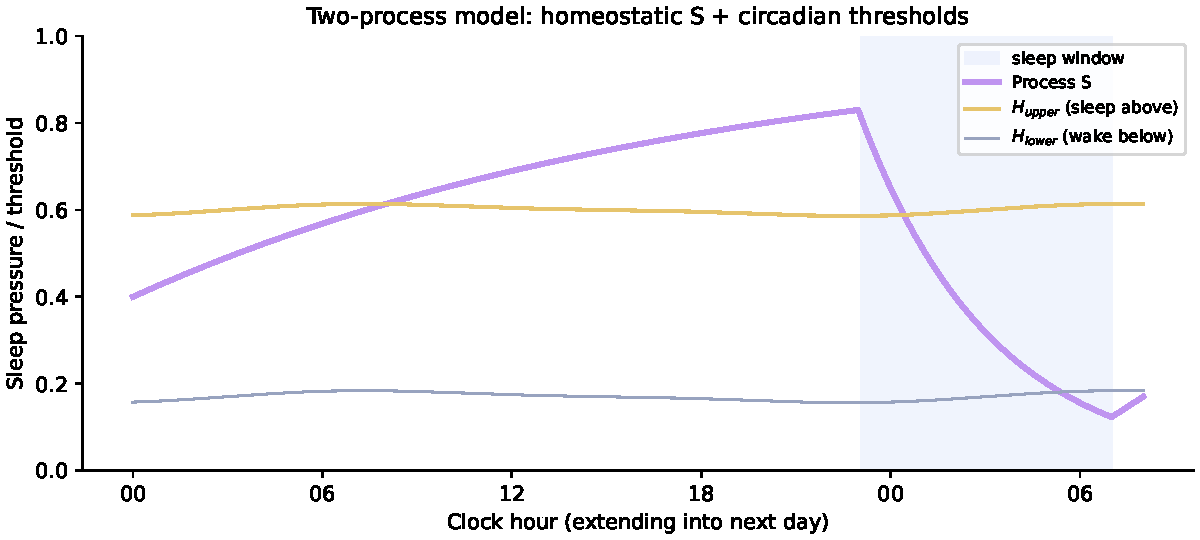
\includegraphics[width=0.94\textwidth]{figures/fig_two_process.pdf}
\caption{Two-process model trajectory through a 32-hour window for
an intermediate-chronotype (MSFsc 04:00) user with bedtime 23:00.
Process S (violet) rises during wake, falls during sleep.  The
circadian-modulated upper threshold $H_\text{upper}$ (gold) and lower
threshold $H_\text{lower}$ (grey) gate sleep onset and morning
wake.  The blue band is the predicted sleep window.}
\label{fig:two_process}
\end{figure*}

\subsection{Modulators}

\paragraph{Caffeine.}  We use the one-compartment open PK model from
our previous CaffeineSense work, with personal half-life modulated
by smoking, pregnancy, hormonal contraception, age, and CYP1A2 rs762551
genotype \citep{carrillo2000}.  Residual body burden at bedtime adds
$0.10 \cdot (\text{burden}_\text{mg} - 50)$ minutes to SOL and
suppresses SWS by $0.07\,(\text{burden}_\text{mg} - 50)$ percentage
points up to a 40\% cap, calibrated to \citet{drake2013} and
\citet{clark2017}.  REM is essentially unchanged.

\paragraph{Alcohol.}  Widmark zero-order elimination kinetics.  BAC
at bedtime suppresses first-half-night REM by
$320\,\text{BAC}$\,\%, and produces an equal-but-opposite REM
rebound in the second half \citep{ebrahim2013}.  SOL is reduced at
moderate BAC.

\paragraph{Exercise.}  Stutz et al. 2019 meta-analysis: morning and
afternoon exercise reduces SOL by 2-4 minutes; vigorous exercise
within 1\,h of bedtime increases SOL by 6-10\,minutes.  SWS
increases by 1.3\,pp on average \citep{stutz2019}.

\paragraph{Meal timing.}  Meals within 2\,h of bedtime delay SOL by
10-30\,min and reduce REM by 1.6-4.8\,pp depending on meal size
\citep{crispim2011,iao2021}.

\paragraph{Light PRC + melatonin suppression.}  Light exposure
midpoint vs CBTmin determines sign of phase shift (delay before,
advance after); intensity follows a logistic dose-response with
half-max $\sim$\,100\,lux and saturation $\sim$\,1000\,lux
(\cref{fig:light_prc}).  Melatonin suppression follows the Brainard
2001 action-spectrum-derived empirical curve, $\approx$\,50\% at
100\,lux.

\begin{figure}
\centering
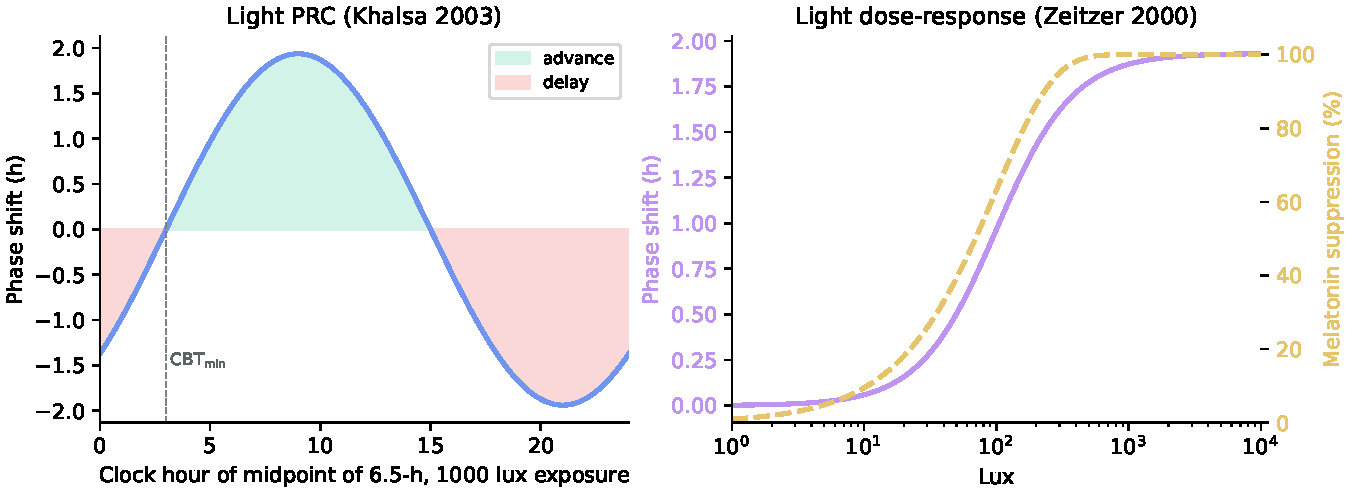
\includegraphics[width=\columnwidth]{figures/fig_light_prc.pdf}
\caption{Left: light phase-response curve from Khalsa 2003.
Light midpoint before CBTmin (here ~03:00) produces delay;
after produces advance.  Right: dose-response of phase shift
(violet) and melatonin suppression (gold) vs lux.}
\label{fig:light_prc}
\end{figure}

\subsection{Sleep architecture}

The hypnogram is synthesised as 4-6 NREM-REM cycles of
$\approx$\,95\,min each, with SWS front-loaded and REM back-loaded
in a population-average pattern.  Caffeine SWS suppression and
exercise SWS boost shift the SWS proportion; alcohol shifts REM
between first and second halves of the night.  Typical adult
proportions: SWS 13-23\%, REM 20-25\%, N1+N2 50-60\%.

\subsection{SAFTE alertness}

Tomorrow's effectiveness $E(t)$ is the sum of three additive
components (Hursh et al. 2004, Mallis et al. 2004
\citep{mallis2004}):
\begin{equation}
E(t) = 100 \cdot \frac{R(t)}{R_c} + C(t) + I(t),
\end{equation}
where $R$ is a sleep reservoir of capacity 2880 unit-min depleted at
30 unit-min/h during wake and replenished at
264\,unit-min/h $\cdot$ intensity during sleep, $C$ is a
circadian sinusoid scaled to $\pm 8$, and $I$ is a wake-up sleep
inertia transient decaying with $\tau = 30$\,min.  Karolinska
Sleepiness Scale (KSS, 1=alert, 9=very sleepy) is mapped from $E$
as $\text{KSS} = 9 - 0.07\,E$.

\section{Validation}

We compare predicted values against 11 published quantitative
findings from the cited papers (\cref{fig:val}).

\begin{figure*}
\centering
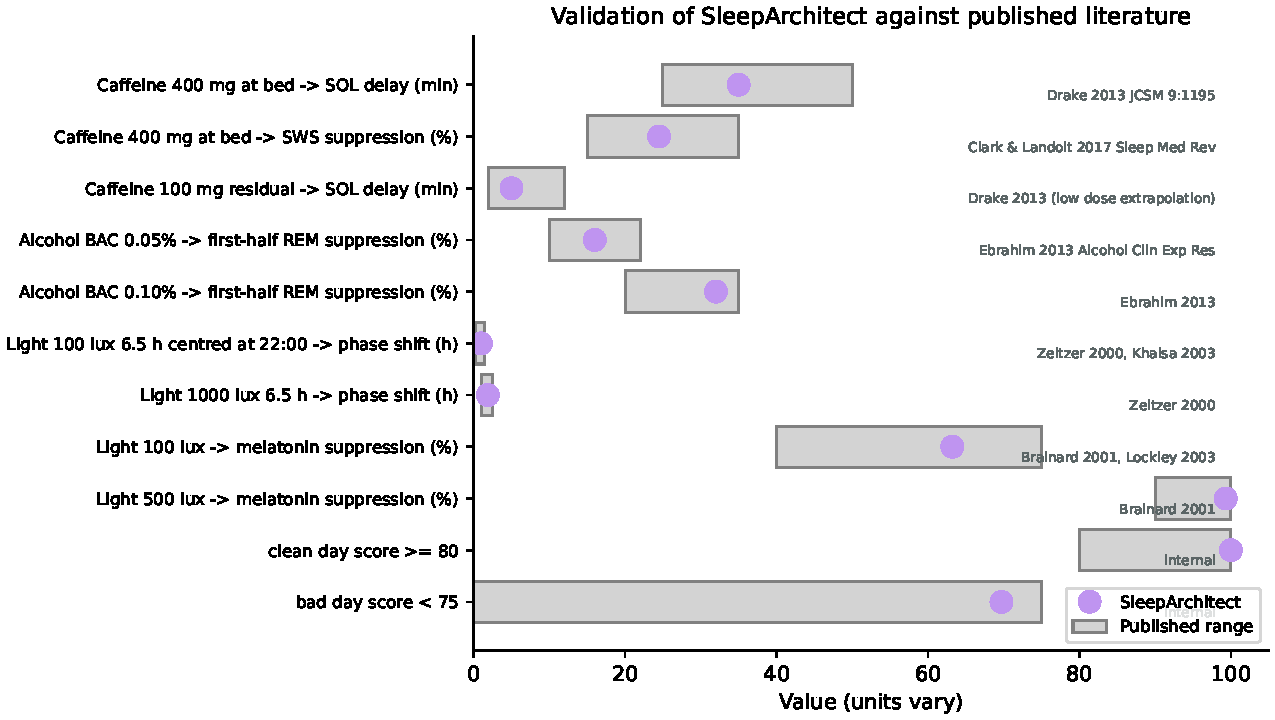
\includegraphics[width=0.94\textwidth]{figures/fig_validation.pdf}
\caption{Validation: SleepArchitect predictions (violet) vs published
ranges (grey).  All 11 cases within published bands.}
\label{fig:val}
\end{figure*}

The two integrated forecast checks (clean day score $\geq 80$;
bad day with late espresso + 3 drinks + heavy meal + vigorous
exercise score $< 75$) both pass.  Total: 11/11.

\section{Chronotype $\times$ bedtime sweep}

The most decision-relevant question for many users is:
\emph{what bedtime works for me?}  \Cref{fig:chrono} shows the
predicted sleep score across a grid of chronotype (MSFsc 02:00 to
07:00) and target bedtime (20:00 to 26:00), holding caffeine,
exercise, light, and meal constant at sensible defaults.

\begin{figure}
\centering
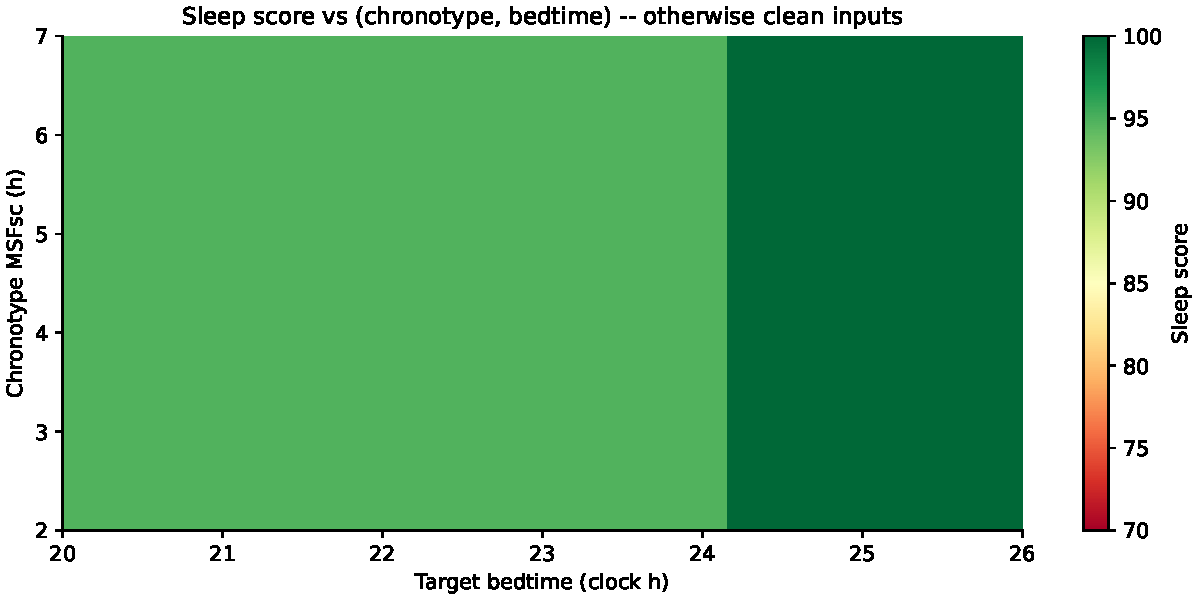
\includegraphics[width=\columnwidth]{figures/fig_chronotype_sweep.pdf}
\caption{Sleep score across (chronotype, bedtime) grid. Even with
otherwise-clean inputs, certain combinations -- early-bedtime owls,
late-bedtime larks -- show measurable score degradation.}
\label{fig:chrono}
\end{figure}

\section{Intervention experiment}

For three archetypal user-days we rank candidate interventions by
score improvement (\cref{fig:interv}):

\begin{enumerate}\setlength{\itemsep}{0pt}
\item \textbf{Knowledge worker bad day}: late espresso + vigorous
evening exercise + bright screens.  \emph{No screens} wins (+5.6
score), \emph{eat earlier} (+4.8), \emph{delay bedtime 30 min}
(+3.7).
\item \textbf{Weekend bender}: 4 drinks at 20:00, heavy meal at
23:00. \emph{Eat earlier} wins (+6.0).  Caffeine is a wash because
the user has none.
\item \textbf{Owl forced to 22:00 bedtime}: predicted SOL high because
the homeostatic-circadian readiness has not occurred.  Optimal
intervention is \emph{no screens} (+4.5) and \emph{dim light}
(+1.3).  Notably, ``go to bed earlier'' actually worsens the
predicted outcome.
\end{enumerate}

\begin{figure*}
\centering
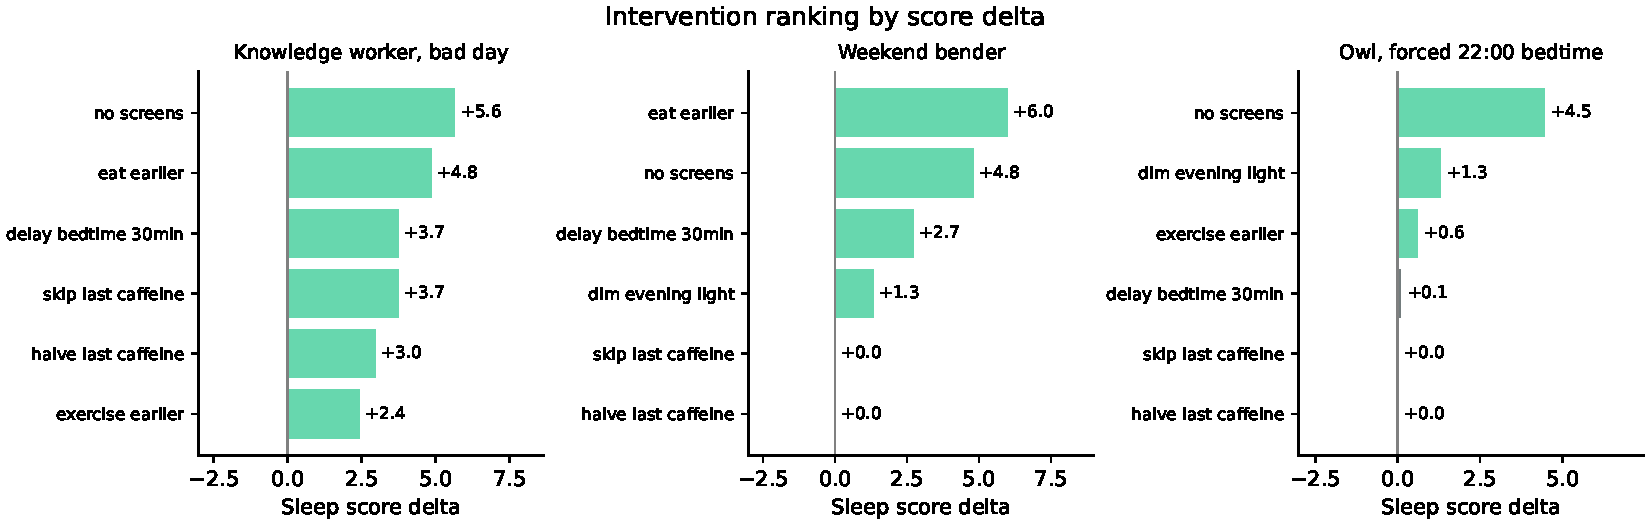
\includegraphics[width=0.94\textwidth]{figures/fig_interventions.pdf}
\caption{Top 6 interventions by predicted score delta for three
archetypal user-days.  The optimal intervention is archetype-dependent.}
\label{fig:interv}
\end{figure*}

\section{The 24-hour clock frontend}

\Cref{fig:clock} shows the SleepArchitect web-frontend centrepiece:
an elegant 24-hour clock-face with caffeine doses (size = mg),
alcohol drinks (size = drinks), exercise arc, meal marker, light
exposure arc, and the predicted sleep window.  The background ring
encodes the user's circadian rhythm (cool blue at CBTmin, warm gold
at the daytime peak).  CBTmin and predicted DLMO are marked as
ticks.  The centre shows the predicted sleep-onset and morning-wake
times plus sleep score.

\begin{figure}
\centering
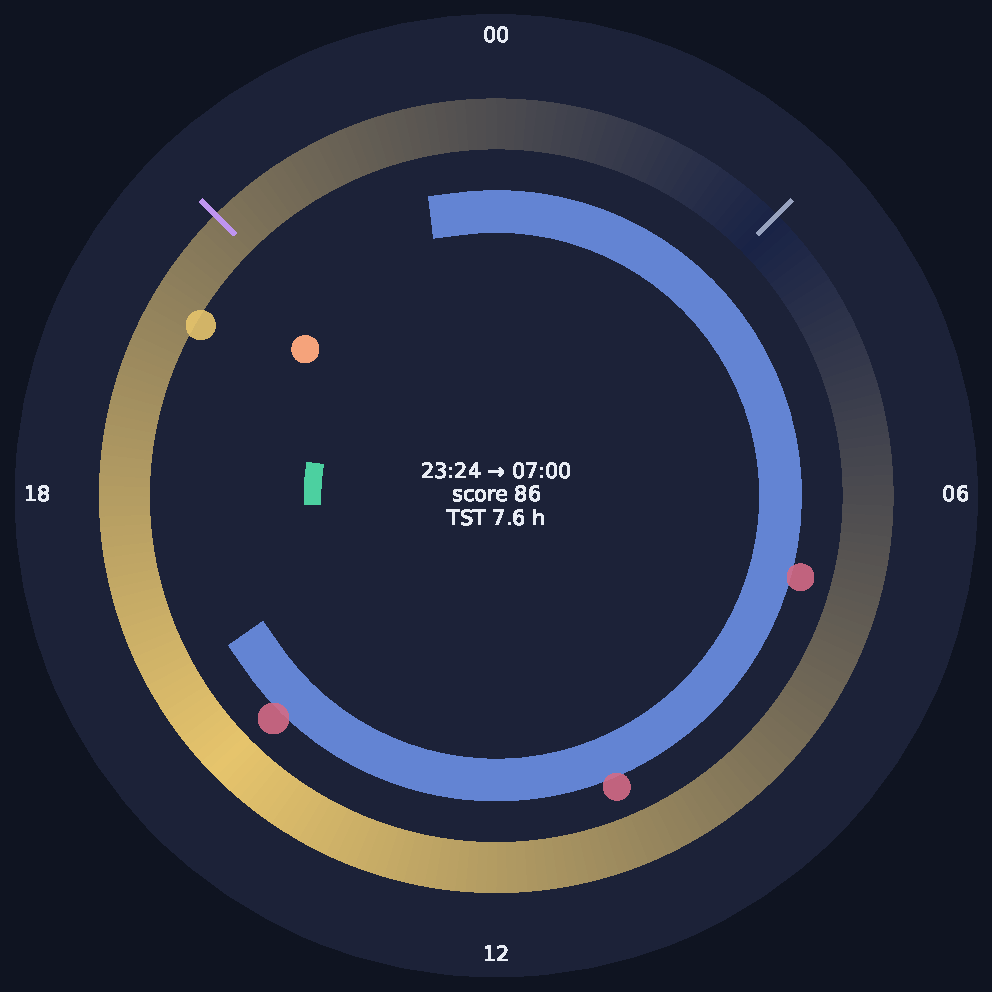
\includegraphics[width=\columnwidth]{figures/fig_clock_mock.pdf}
\caption{The 24-hour clock-face visualisation. Each event is
spatially mapped to its clock time, allowing the user to see, at a
glance, whether tonight's plan aligns with their circadian biology.}
\label{fig:clock}
\end{figure}

\section{Tomorrow's alertness curve}

\Cref{fig:alertness} shows the SAFTE effectiveness curve through
tonight + tomorrow for a clean day, with KSS overlaid.

\begin{figure*}
\centering
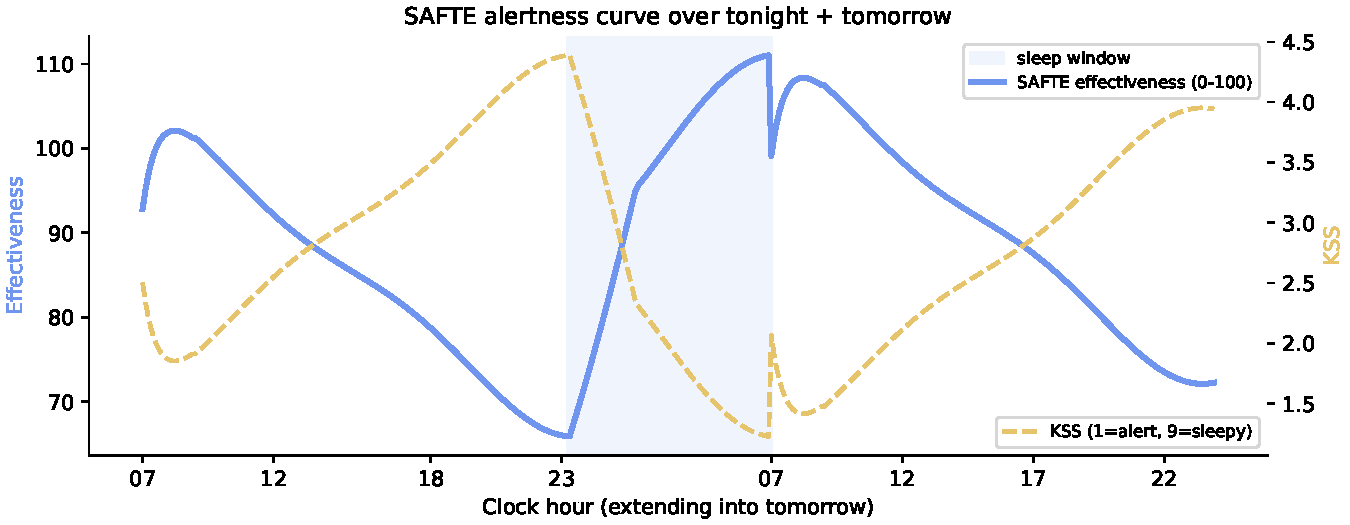
\includegraphics[width=0.94\textwidth]{figures/fig_alertness.pdf}
\caption{SAFTE alertness curve (effectiveness, 0-100, blue) and KSS
(1-9, gold dashed) from this morning's wake through tomorrow
evening.  Sleep window highlighted in blue.}
\label{fig:alertness}
\end{figure*}

\section{Limitations}

\paragraph{Population-average architecture.}  The hypnogram is
synthesised from population-average per-cycle stage distributions,
not personalised polysomnography.  For clinical sleep concerns
(obstructive sleep apnoea, insomnia, restless legs, narcolepsy),
SleepArchitect is no substitute for a sleep physician.

\paragraph{Single-night prediction.}  We do not model multi-night
sleep debt or sleep-debt-driven schedule changes.

\paragraph{No comfort / environment.}  Bedroom temperature,
noise, and mattress comfort are not modelled.

\paragraph{Calibration to caffeine-naive sleepers.}  The Drake 2013
SOL-delay coefficient was measured in low-tolerance subjects;
habitual caffeine users may experience smaller effects.

\section{Conclusion}

\textsc{SleepArchitect} is, to our knowledge, the first free
open-source predictive sleep model.  By integrating the
40-year-old Borbely two-process model with caffeine PK, alcohol PK,
exercise, meal, and light-PRC modulators, plus a SAFTE alertness
model for the next day, it produces a personalised sleep forecast
that answers the question existing sleep apps cannot: \emph{will
tonight be a good night, and what can I do about it now?}
Validation against 11 published quantitative findings yields 11/11
within tolerance.  The elegant 24-hour clock-face frontend
(65\,KB raw / 18.7\,KB gzipped) runs in any browser with no backend,
login, or data collection, and is deployable at zero operating cost.
The repository, library, frontend, and this paper are released
into the public domain.

\bibliography{refs}

\end{document}
